\documentclass{book}
\usepackage{minted}
\usepackage{tikz}
\usepackage{wrapfig}
\usepackage{fancyhdr}
\usepackage{geometry}
\usepackage{calc}
\usepackage{sectsty}
\usepackage{parskip}
%\usepackage{graphicx}
%\graphicxpath{".\images\"}
\geometry{inner=1.2in,outer=1.2in,top=0.75in,bottom=0.75in}
%6502 Assembly Language Programming (2nd Edition)
\chapterfont{\centering\Huge}
\sectionfont{\centering}
\pagestyle{fancy}
\fancyhead{}
\fancyfoot[C]{\thechapter-\thepage}
\begin{document}

\chapter{INTRODUCTION TO ASSEMBLY\\ LANGUAGE PROGRAMMING}

\textbf{This book describes assembly language programming. It assumes that you are familiar with \underline{An Introduction To Microcomputers: Volume 1 - Basic Concepts\textsuperscript{1}} (particularly Chapters 6 and 7). This book does not discuss the general features of computers, microcomputers, addressing methods, or instruction sets; you should refer to \underline{An Introduction To Microcomputers: Volume 1} for that information.}

\subsection*{HOW THIS BOOK HAS BEEN PRINTED}

\textbf{Notice that text in this book has been printed in boldface type and lightface type. This has been done to help you skip those parts of the book that cover subject matter with which you are familiar. You can be sure that lightface type only expands on information presented in the previous boldface type.} Therefore. only read boldface type until you reach a subject about which you want to know more. at which point start reading the lightface type.

\section*{THE MEANING OF INSTRUCTIONS}

\textbf{The instruction set of a microprocessor is the set of binary inputs that produce defined actions during an instruction cycle.} An instruction set is to a microprocessor what a function table is to a logic device. such as a gate. adder. or shift register. Of course. the actions that the microprocessor performs in response to its instruction inputs are far more complex than the actions that logic devices perform in response to their inputs.\\
\begin{wrapfigure}{r}{3.2cm+.6666em+.8pt}

\begin{tikzpicture}[every node/.style={draw,ultra thick,text width=3.2cm,minimum width=3.2cm}]
\node{\textbf{BINARY\\ INSTRUCTIONS}};
\end{tikzpicture}
\end{wrapfigure}
\textbf{An instruction is a binary bit pattern - it must be available at the data inputs to the microprocessor at the proper time in order to be interpreted as an instruction.} For example. when the 6502 microprocessor receives the 8-bit binary pattern 11101000 as the input during an instruction fetch operation. the pattern means:\\

"Increment (add 1 to) the contents of Register X".\\

Similarly. the pattern 10101001 means:\\

"Load the Accumulator with the contents of the next word of program memory".\\

The microprocessor (like any other computer) recognizes only binary patterns as instructions or data: it does not recognize words or octal. decimal. or hexadecimal numbers.

\subsection*{A COMPUTER PROGRAM}
\textbf{A program is a series of instructions that causes a computer to perform a particular task.}\\
\begin{wrapfigure}{r}{2.2cm+.6666em+.8pt}

\begin{tikzpicture}[every node/.style={draw,ultra thick,text width=2.2cm,minimum width=2.2cm}]
\node{\textbf{COMPUTER\\ PROGRAM}};
\end{tikzpicture}
\end{wrapfigure}
Actually. a computer program includes more than instructions; it also contains the data and memory addresses that the microprocessor needs to accomplish the tasks defined by the instructions. Clearly. if the microprocessor is to perform an addition. it must have two numbers to add and a place to put the result. The computer program must determine the sou rces of the data and the destination of the resu It as well as the operation to be performed.

All microprocessors execute instructions sequentially unless one of the instructions changes the execution sequence or halts the computer. i.e.. the processor gets the next instruction from the next consecutive memory address unless the current instruction specifically directs it to do otherwise.\\

\textbf{Ultimately every program is translated into a set of binary numbers. For example, this is a 6502 program that adds the contents of memory locations 0060\textsubscript{16} and 0061\textsubscript{16} and places the result in memory location 0062\textsubscript{16}:}\\

\begin{center}
10100101\\
01100000\\
01100101\\
01100001\\
10000101\\
01100010\\
\end{center}


\begin{wrapfigure}{r}{2.4cm+.6666em+.8pt}

\begin{tikzpicture}[every node/.style={draw,ultra thick,text width=2.4cm,minimum width=2.4cm}]
\node{\textbf{OBJECT\\ PROGRAM}};
\end{tikzpicture}

\begin{tikzpicture}[every node/.style={draw,ultra thick,text width=2.4cm,minimum width=2.4cm}]
\node{\textbf{MACHINE\\ LANGUAGE\\ PROGRAM}};
\end{tikzpicture}
\end{wrapfigure}
\noindent\textbf{This is a machine language, or object, program.} If this program were entered into the memory of a 6502-based microcomputer. the microcomputer would be able to execute it directly.\\

\subsection*{THE PROGRAMMING PROBLEM}

\textbf{There are many difficulties associated with creating programs as object, or binary machine language, programs. These are some of the problems:}\\

\begin{enumerate}
     \item {The programs are difficult to understand or debug (binary numbers all look the same. particularly after you have looked at them for a few hours).}
     \item {The programs are slow to enter since you nust determine each bit individually.}
     \item {The programs do not describe the task which you want the computer to perform in anything resembling a human readable format.}
     \item {The programs are long and tiresome to write.}
     \item {The programmer often makes careless errors that are very difficult to locate and correct.}
\end{enumerate}

For example. \textbf{the following version of the addition object program contains a single bit error. Try to find it:}
\begin{center}
10100101\\
01100000\\
01110101\\
01100001\\
10000101\\
01100010
\end{center}
Although the computer handles binary numbers with ease. people do not. People find binary programs long. tiresome. confusing. and meaningless. Eventually. a programmer may start remembering some of the binary codes. but such effort should be spent more productively.

\subsection*{USING OCTAL OR HEXADECIMAL}
\begin{wrapfigure}{r}{3.2cm+.6666em+.8pt}

\begin{tikzpicture}[every node/.style={draw,ultra thick,text width=3.2cm,minimum width=3.2cm}]
\node{\textbf{OCTAL OR\\ HEXADECIMAL}};
\end{tikzpicture}
\end{wrapfigure}
\textbf{We can improve the situation somewhat by writing instructions using octal or hexadecimal, rather than binary numbers.} We will use hexadecimal numbers in this book because they are shorter. and because they are the standard for the microprocessor industry. Table 1-1 defines the hexadecimal digits and their binary equivalents. \textbf{The 6502 program to add two numbers now becomes:}

\begin{center}
A5\\
60\\
65\\
61\\
85\\
62
\end{center}
At the very least. the hexadecimal version is shorter to write and not quite so tiring to examine.

\textbf{Errors are somewhat easier to find in a sequence of hexadecimal digits. The erroneous version of the addition program, in hexadecimal form, becomes:}
\begin{center}
A5\\
60\\
75\\
61\\
85\\
62
\end{center}
\textbf{The mistake is far more obvious.}

\textbf{What do we do with this hexadecimal program? The microprocessor understands only binary instruction codes.} The answer is that we must convert the hexadecimal numbers to binary numbers. This conversion is a repetitive. tiresome task. People who attempt it make all sorts of petty mistakes. such as looking at the wrong line. dropping a bit. or transposing a bit or a digit.

\begin{wrapfigure}{r}{3.2cm+.6666em+.8pt}
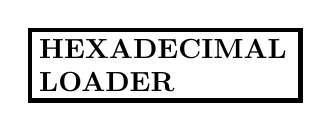
\begin{tikzpicture}[every node/.style={draw,ultra thick,text width=3.2cm,minimum width=3.2cm}]
\node{\textbf{HEXADECIMAL\\ LOADER}};
\end{tikzpicture}
\end{wrapfigure}
This repetitive. grueling task is. however. a perfect job for a computer. The computer never gets tired or bored and never makes silly mistakes. \textbf{The idea then is to write a program that accepts hexadecimal numbers and converts them into binary numbers. This is a standard program provided with many microcomputers; it is called a hexadecimal loader.}

Is a hexadecimal loader worth having? If you are willing to write a program using binary numbers. and you are prepared to enter the program in its binary form into the computer. then you will not need the hexadecimal loader.

If you choose the hexadecimal loader. you will have to pay a price for it The hexadecimal loader is itself a program that you must load into memory. Furthermore. the hexadecimal loader will occupy memory - memory that you may want to use in some other way.

The basic tradeoff. therefore. is the cost and memory requirements of the hexadecimal loader versus the savings in programmer time.

A hexadecimal loader is well worth its small cost.

A hexadecimal loader certainly does not solve every programming problem. The hexadecimal version of the program is still difficult to read or understand: for example. it does not distinguish instructions from data or addresses. nor does the program listing provide any suggestion as to what the program does. What does 85 or DO mean? Memorizing a card full of codes is hardly an appetizing proposition. Furthermore. the codes will be entirely different for a different microprocessor. and the program will require a large amount of documentation.

\begin{table}[H]
     \begin{center}
          \caption{Hexadecimal Conversion Table}
          \label{tab:11}
          \begin{tabular}{|c|c|c|}
               \hline
               \begin{tabular}[c]{@{}c@{}}Hexadecimal\\ Digit\end{tabular} & \begin{tabular}[c]{@{}c@{}}Binary\\ Equivalent\end{tabular} & \begin{tabular}[c]{@{}c@{}}Decimal\\ Equivalent\end{tabular} \\ \hline
               0 & 0000 & 0 \\
               1 & 0001 & 1 \\
               2 & 0010 & 2 \\
               3 & 0011 & 3 \\
               4 & 0100 & 4 \\
               5 & 0101 & 5 \\
               6 & 0110 & 6 \\
               7 & 0111 & 7 \\
               8 & 1000 & 8 \\
               9 & 1001 & 9 \\
               A & 1010 & 10 \\
               B & 1011 & 11 \\
               C & 1100 & 12 \\
               D & 1101 & 13 \\
               E & 1110 & 14 \\
               F & 1111 & 15 \\ \hline
          \end{tabular}
     \end{center}
\end{table}

\subsection*{INSTRUCTION CODE MNEMONICS}
\textbf{An obvious programming improvement is to assign a name to each instruction code. The instruction code name is called a "mnemonic" or memory jogger. The instruction mnemonic should describe in some way what the instruction does.}\\

\begin{wrapfigure}{r}{2.6cm+.6666em+.8pt}
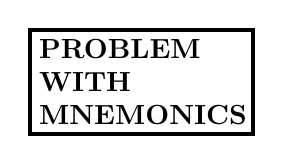
\begin{tikzpicture}[every node/.style={draw,ultra thick,text width=2.6cm,minimum width=2.6cm}]
\node{\textbf{PROBLEM\\ WITH\\ MNEMONICS}};
\end{tikzpicture}
\end{wrapfigure}
In fact. every microprocessor manufacturer (they can't remember hexadecimal codes either) provides a set of mnemonics for the microprocessor instruction set. \textbf{You do not have to abide by the manufacturer's mnemonics;} there is nothing sacred about them.

However. they are standard for a given microprocessor and therefore understood by all users. These are the instruction codes that you will find in manuals. cards. books. articles. and programs. The problem with selecting instruction mnemonics is that not all instructions have "obvious" names. Some instructions do (e.g.. ADD. AND. OR). others have obvious contractions (e.g.. SUB for subtraction. XOR for exclusive-OR). while still others have neither. The result is such mnemonics as WMP. PCHL. and even SOB (guess what that means!). Most manufacturers come up with some reasonable names and some hopeless ones. However. users who devise their own mnemonics rarely do much better than the manufacturer.

Along with the instruction mnemonics. the manufacturer will usually assign names to the CPU registers. As with the instruction names. some register names are obvious (e.g.. A for Accumulator) while others may have only historical significance. Again. we will use the manufacturer's suggestions simply to promote standardization.\\

\begin{wrapfigure}{r}{2.4cm+.6666em+.8pt}

\begin{tikzpicture}[every node/.style={draw,ultra thick,text width=2.4cm,minimum width=2.4cm}]
\node{\textbf{ASSEMBLY\\ LANGUAGE\\ PROGRAM}};
\end{tikzpicture}
\end{wrapfigure}
\textbf{If we use standard 6502 instruction and register mnemonics, as defined by MOS Technology, Inc., our 6502 addition program becomes:}
\begin{minted}{ca65}
LDA $60
ADC $61
STA $62
\end{minted}

The program is still far from obvious. but at least some parts are comprehensible. ADC is a considerable improvement over 65; LDA and STA suggest loading and storing the contents of the Accumulator. We now know which lines are instructions and which are data or addresses. \noindent \textbf{Such a program is an assembly language program.}

\subsection*{THE ASSEMBLER PROGRAM}

\begin{wrapfigure}{r}{2.2cm+.6666em+.8pt}

\begin{tikzpicture}[every node/.style={draw,ultra thick,text width=2.2cm,minimum width=2.2cm}]
\node{\textbf{HAND\\ ASSEMBLY}};
\end{tikzpicture}
\end{wrapfigure}
How do we get the assembly language program into the computer? We have to translate it. either into hexadecimal or into binary numbers. \textbf{You can translate an assembly language program by hand,} instruction by instruction. This is called hand assembly.

Hand assembly of the addition program may be illustrated as follows:
\begin{table}[H]
\begin{tabular}{ccc}
Instruction Mnemonic & Addressing Method & Hexadecimal Equivalent \\ \hline
LDA & Zero Page (direct) & A5 \\
ADC & Zero Page (direct) & 65 \\
STA & Zero Page (direct) & 85
\end{tabular}
\end{table}
As with hexadecimal to binary conversion. hand assembly is a rote task which is uninteresting. repetitive, and subject to numerous minor errors. Picking the wrong line, transposing digits, omitting instructions, and misreading the codes are only a few of the mistakes that you may make. Most microprocessors complicate the task even further by having instructions with different word lengths. Some instructions are one word long while others are two or three words long. Some instructions require data in the second and third words. others require memory addresses. register numbers. or who knows what?\\
\begin{wrapfigure}{r}{2.5cm+.6666em+.8pt}

\begin{tikzpicture}[every node/.style={draw,ultra thick,text width=2.5cm,minimum width=2.5cm}]
\node{\textbf{ASSEMBLER}};
\end{tikzpicture}

\begin{tikzpicture}[every node/.style={draw,ultra thick,text width=2.5cm,minimum width=2.5cm}]
\node{\textbf{SOURCE\\ PROGRAM}};
\end{tikzpicture}

\begin{tikzpicture}[every node/.style={draw,ultra thick,text width=2.5cm,minimum width=2.5cm}]
\node{\textbf{OBJECT\\ PROGRAM}};
\end{tikzpicture}
\end{wrapfigure}
\textbf{Assembly is another rote task that we can assign to the microcomputer. The microcomputer never makes any mistakes when translating codes; it always knows how many words and what format each instruction requires. The program that does this job is an "assembler." The assembler program translates a user program, or "source" program written with mnemonics, into a machine language program, or "object" program, which the microcomputer can execute. The assembler's input is a source program and its output is an object program.}\\

\textbf{The tradeoffs that we discussed in connection with the hexadecimal loader are magnified in the case of the assembler.} Assemblers are more expensive. occupy more memory. and require more peripherals and execution time than do hexadecimal loaders. While users may (and often do) write their own loaders. few care to write their own assemblers.\\

\textbf{Assemblers have their own rules that you must learn.} These include the use of certain markers (such as spaces. commas. semicololls. or colons) in appropriate places. correct spelling. the proper control information. and perhaps even the correct placement of names and numbers. These rules are usually simple and can be learned quickly. 

\subsection*{ADDITIONAL FEATURES OF ASSEMBLERS}

Early assemblers did little more than translate the mnemonic names of instructions and
registers into their binary equivalents. However. most assemblers now provide such additiona I featu res as:
\begin{enumerate}
\item{Allowing the user to assign names to memory locations. input and output devices. and even sequences of instructions.}
\item{Converting data or addresses from various number systems (e.g.. decimal or hexadecimal) to binary and converting characters into their ASCII or EBCDIC binary codes.}
\item{Performing some arithmetic as part of the assembly process.}
\item{Telling the loader program where in memory parts of the program or data should be placed.}
\item{Allowing the user to assign areas of memory as temporary data storage and to place fixed data in areas of program memory.}
\item{Providing the information required to include standard programs from program libraries. or programs written at some other time. in the current program.}
\item{Allowing the user to control the format of the program listing and the input and output devices employed.}
\end{enumerate}

\begin{wrapfigure}{r}{2.5cm+.6666em+.8pt}
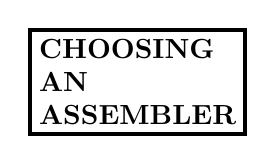
\begin{tikzpicture}[every node/.style={draw,ultra thick,text width=2.5cm,minimum width=2.5cm}]
\node{\textbf{CHOOSING\\ AN\\ ASSEMBLER}};
\end{tikzpicture}
\end{wrapfigure}
All of these features. of course. involve additional cost and memory. Microcomputers generally have much simpler assemblers than do larger computers. but the tendency always is for the size of assemblers to increase. You will often have a choice of assemblers.\\
The important criterion is not how many offbeat features the assembler has. but rather
how convenient it is to work with in normal practice.

\subsection*{DISADVANTAGES OF ASSEMBLY LANGUAGE}
\textbf{The assembler. like the hexadecimal loader. does not solve all the problems of programming. One problem is the tremendous gap between the microcomputer instruction set and the tasks which the microcomputer is to perform.} Computer instructions tend to do things like add the contents of two registers. shift the contents of the Accumulator one bit. or place a new value in the Program Counter. On the other hand. a user generally wants a microcomputer to do something like check if an analog reading has exceeded a threshold. look for and react to a particular command from a teletypewriter. or activate a relay at the proper time. An assembly language programmer must translate such tasks into a sequence of simple computer instructions. The translation can be a difficult. time-consuming job.

Fu rthermore, \textbf{if you are programming in assembly language. you must have detailed knowledge of the particular microcomputer that you are using.} You must know what registers and instructions the microcomputer has. precisely how the instructions affect the various registers. what addressing methods the computer uses. and a myriad of other information. None of this information is relevant to the task which the microcomputer must ultimately perform.

\begin{wrapfigure}{r}{2.8cm+.6666em+.8pt}

\begin{tikzpicture}[every node/.style={draw,ultra thick,text width=2.8cm,minimum width=2.8cm}]
\node{\textbf{PORTABILITY}};
\end{tikzpicture}
\end{wrapfigure}
\textbf{In addition. assembly language programs are not portable.} Each microcomputer has its own assembly language. which reflects its own architecture. An assembly language program written for the 6502 will not run on a 6800. Z80. 8080. or 3870 microprocessor. For example. the addition program written for the 8080 would be:
\begin{minted}{ca65}
LDA 60H
MOV B.A
LDA 61H
ADD B
STA 62H
\end{minted}
The lack of portability not only means that you won't be able to use your assembly
language program on another microcomputer. but it also means that you won't be able
to use any programs that weren't specifically written for the microcomputer you are
using, This is a particular drawback for microcomputers, since these devices are new
and few assembly language programs exist for them. The result. too frequently, is that
you are on your own. If you need a program to perform a particular task, you are not
likely to find it in the small program libraries that most manufacturers provide. Nor are
you likely to find it in an archive, journal article. or someone's old program file. You will
probably have to write it yourself.

\subsection*{HIGH-LEVEL LANGUAGES}
\begin{wrapfigure}{r}{2.2cm+.6666em+.8pt}

\begin{tikzpicture}[every node/.style={draw,ultra thick,text width=2.2cm,minimum width=2.2cm}]
\node{\textbf{COMPILER}};
\end{tikzpicture}
\end{wrapfigure}
\textbf{The solution to many of the difficulties associated with assembly language programs is to use. instead. “high-level” or “procedure-oriented” languages, Such languages allow you to describe tasks in forms that are problem oriented rather than computer oriented. Each statement in a high-level language performs a recognizable function; it will generally correspond to many assembly language instructions. A program called a compiler translates the high-level language source program into object code or machine language instructions.}

\begin{wrapfigure}{r}{2cm+.6666em+.8pt}

\begin{tikzpicture}[every node/.style={draw,ultra thick,text width=2cm,minimum width=2cm}]
\node{\textbf{FORTRAN}};
\end{tikzpicture}
\end{wrapfigure}
Many different high·level languages exist for different types of tasks. If, for example, you can express what you want the computer to do in algebraic notation, you can write your program in FORTRAN (Formula Translation Language). the oldest and most widely used of the high-level languages. Now, if you want to add two numbers, you just tell the computer:
\begin{center}
SUM = NUMB1 + NUMB2
\end{center}
That is a lot simpler (and a lot shorter) than either the equivalent machine language program or the equivalent assembly language program. Other high-level languages include COBOL (for business applications). PASCAL (another algebraic language). PL/1 (a combination of FORTRAN, ALGOL. and COBOL), and APL and BASIC (languages that are popular for time-sharing systems).

\subsection*{ADVANTAGES OF HIGH-LEVEL LANGUAGES}

\textbf{Clearly. high-level languages make programs easier and faster to write, A common estimate is that a programmer can write a program about ten times as fast in a high-level language as compared to assembly language.\textsuperscript{1-3}} That is just writing the program; it does not include problem definition, program design, debugging, testing, or documentation, all of which become simpler and faster. The high-level language program is, for instance, partly self-documenting. Even if you do not know FORTRAN. you probably could tell what the statement illustrated above does.

\begin{wrapfigure}{r}{3.2cm+.6666em+.8pt}

\begin{tikzpicture}[every node/.style={draw,ultra thick,text width=3.4cm,minimum width=3.4cm}]
\node{\textbf{MACHINE\\ INDEPENDENCE\\ OF HIGH-LEVEL\\ LANGUAGES}};
\end{tikzpicture}
\end{wrapfigure}
\textbf{High-level languages solve many other problems associated with assembly language programming.} The high-level language has its own syntax (usually defined by a national or international standard). The language does not mention the instruction set. registers, or other features of a particular computer. The compiler takes care of all such details. Programmers (;an concentrate on their own tasks; they do not need a detailed understanding of the underlying CPU architecture - for that matter, they do not need to know anything about the computer they are
programming.

\begin{wrapfigure}{r}{3.2cm+.6666em+.8pt}

\begin{tikzpicture}[every node/.style={draw,ultra thick,text width=3.4cm,minimum width=3.4cm}]
\node{\textbf{PORTABILITY\\ OF HIGH-LEVEL\\ LANGUAGES}};
\end{tikzpicture}
\end{wrapfigure}
\textbf{Programs written in a high-level language are portableat least. in theory.} They will run on any computer that has a standard compiler for that language. 

At the same time. all previous programs written in a high-level language for prior computers are available to you when programming a new computer. This can mean thousands of programs in the case of a common language like FORTRAN or BASIC.

\subsection*{DISADVANTAGES OF HIGH-LEVEL LANGUAGES}
\textbf{Well, if all the good things we have said about high-level languages are true, if you can write programs faster and make them portable besides, why bother with assembly languages? Who wants to worry about registers, instruction codes, mnemonics, and all that garbage! As usual, there are disadvantages that balance the advantages.}

\begin{wrapfigure}{r}{2.8cm+.6666em+.8pt}
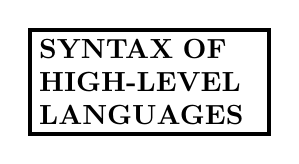
\begin{tikzpicture}[every node/.style={draw,ultra thick,text width=2.8cm,minimum width=2.8cm}]
\node{\textbf{SYNTAX OF\\ HIGH-LEVEL\\ LANGUAGES}};
\end{tikzpicture}
\end{wrapfigure}
One obvious problem is that \textbf{you have to learn the "rules" or "syntax" of any high-level language} you want to use. A highlevel language has a fairly complicated set of rules. You will find that it takes a lot of time just to get a program that is syntactically correct (and even then it probably will not do what you want!' A high-level computer language is like a foreign language. If you have a little talent. you will get used to the rules and be able to turn out programs that the compiler will accept. Still. learning the rules and trying to get the program accepted by the compiler does not contribute directly to doing your job.

Here. for example. are some FORTRAN rules:
\begin{itemize}
\item{Labels must be numbers placed in the first five card columns}
\item{Statements must start in column seven}
\item{Integer variables must start with the letters I. J. K. L. M. or N}
\end{itemize}

\begin{wrapfigure}{r}{2.4cm+.6666em+.8pt}

\begin{tikzpicture}[every node/.style={draw,ultra thick,text width=2.4cm,minimum width=2.4cm}]
\node{\textbf{COST OF\\ COMPILERS}};
\end{tikzpicture}
\end{wrapfigure}
Another obvious problem is that you need a compiler to translate programs written in a high-level language. Compilers are expensive and use a large amount of memory. While most assemblers occupy 2K to 16K bytes of memory (1 K = 1024). compilers occupy 4K to 64K bytes. So the amount of overhead involved in using the compiler is rather large.

\begin{wrapfigure}{r}{2.4cm+.6666em+.8pt}

\begin{tikzpicture}[every node/.style={draw,ultra thick,text width=2.4cm,minimum width=2.4cm}]
\node{\textbf{ALGEBRAIC\\ NOTATION}};
\end{tikzpicture}
\end{wrapfigure}
Furthermore. \textbf{only some compilers will make the implementation of your task simpler.} FORTRAN, for example, is well-suited to problems that can be expressed as algebraic formulas. If, however, your problem is controlling a printer, editing a string of characters. or monitoring an alarm system, your problem cannot be easily expressed in algebraic notation. In fact. formulating the solution in algebraic notation may be more awkward and more difficult than formulating it in assembly language. One answer is to use a more suitable high-level language. Some such languages exist. but they are far less widely used and standardized than FORTRAN. You will not get many of the advantages of high-level languages if you use these so-called system implementation languages.

\begin{wrapfigure}{r}{3cm+.6666em+.8pt}
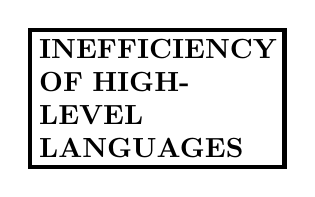
\begin{tikzpicture}[every node/.style={draw,ultra thick,text width=3cm,minimum width=3cm}]
\node{\textbf{INEFFICIENCY\\ OF HIGH-LEVEL\\ LANGUAGES}};
\end{tikzpicture}

\begin{tikzpicture}[every node/.style={draw,ultra thick,text width=3cm,minimum width=3cm}]
\node{\textbf{OPTIMIZING\\ COMPILER}};
\end{tikzpicture}
\end{wrapfigure}
\textbf{High-level languages do not produce very efficient machine language programs.} The basic reason for this is that compilation is an automatic process which is riddled with compromises to allow for many ranges of possibilities. The compiler works much like a computerized language translator -- sometimes the words are right but the sounds and sentence structures are awkward, A Simple compiler cannot know when a variable is no longer being used and can be discarded, when a register should be used rather than a memory location, or when variables have simple relationships. The experienced programmer can take advantage of shortcuts to shorten execution time or reduce memory usage. A few compilers (known as optimizing compilers) can also do this. but such compilers are much larger and slower than regular compilers.

The general advantages and disadvantages of high-level languages are:
\begin{wrapfigure}{r}{2.8cm+.6666em+.8pt}
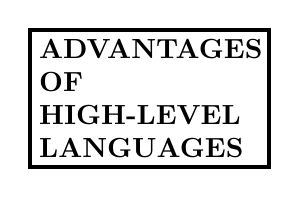
\begin{tikzpicture}[every node/.style={draw,ultra thick,text width=2.8cm,minimum width=2.8cm}]
\node{\textbf{ADVANTAGES\\ OF\\ HIGH-LEVEL\\ LANGUAGES}};
\end{tikzpicture}
\end{wrapfigure}
\textbf{Advantages:}
\begin{wrapfigure}{r}{3.8cm+.6666em+.8pt}
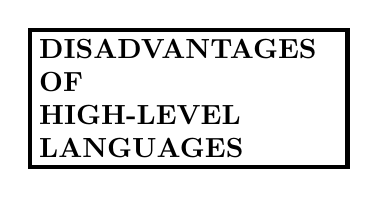
\begin{tikzpicture}[every node/.style={draw,ultra thick,text width=3.8cm,minimum width=3.8cm}]
\node{\textbf{DISADVANTAGES\\ OF\\ HIGH-LEVEL\\ LANGUAGES}};
\end{tikzpicture}
\end{wrapfigure}
\begin{itemize}
\item{More convenient descriptions of tasks}
\item{Less time spent writing programs}
\item{Easier documentation}
\item{Standard syntax}
\item{Independence of the structure of a particular computer}
\item{Portability}
\item{Availability of library and other programs}
\end{itemize}

\textbf{Disadvantages:}
\begin{itemize}
\item{Special rules}
\item{Extensive hardware and software support required}
\item{Orientation of common languages to algebraic or business problems}
\item{Inefficient programs}
\item{Difficulty of optimizing code to meet time and memory requirements}
\item{Inability to use special features of a computer conveniently}
\end{itemize}

\subsection*{HIGH-LEVEL LANGUAGES FOR MICROPROCESSORS}

\textbf{Microprocessor users will encounter several special difficulties when using highlevel languages. Among these are:}
\begin{itemize}
\item\textbf{Few high-level languages exist for microprocessors}
\item\textbf{Few standard languages are widely available}
\item\textbf{Compilers usually require a large amount of memory or even a completely different computer}
\item\textbf{Most microprocessor applications are not well-suited to high-level languages}
\item\textbf{Memory costs are often critical in microprocessor applications}
\end{itemize}
The lack of high-level languages is partly a result of the fact that microprocessors are quite new and are the products of semiconductor manufacturers rather than computer manufacturers. Very few high-level languages exist for microprocessors. The most common are BASIC,\textsuperscript{5} PASCAL,\textsuperscript{6} FORTRAN, and the PL/I-type languages such as PL/M.\textsuperscript{7} MPL, and PL/$\mu$S.

Many of the high-level languages that exist do not conform to recognized standards. so that the microprocessor user cannot expect to gain much program portability. access to program libraries. or use of previous experience or programs. The main advantages remaining are the reduction in programming effort and the smaller amount of detailed understanding of the computer architecture that is necessary.

\begin{wrapfigure}{r}{3cm+.6666em+.8pt}
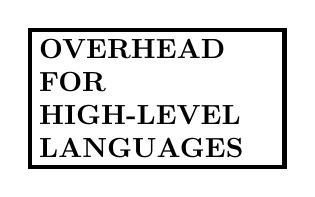
\begin{tikzpicture}[every node/.style={draw,ultra thick,text width=3cm,minimum width=3cm}]
\node{\textbf{OVERHEAD\\ FOR\\ HIGH-LEVEL\\ LANGUAGES}};
\end{tikzpicture}
\end{wrapfigure}
The overhead involved in using a high-level language with microprocessors is considerable. Microprocessors themselves are better suited to control and slow interactive applications than they are to the character manipulation and language analysis involved in compilation. Therefore. some compilers for microprocessors will not run on a microprocessor-based system. Instead. they require a much larger computer; i.e.. they are cross-compilers rather than self-compilers. A user must not only bear the expense of the larger computer but must also physically transfer the program from the larger computer to the micro.

Some self-compilers are available. These compilers run on the microcomputer for which they produce object code. Unfortu nately. they require large amounts of memory (16K or morel. plus special supporting hardware and software.

\begin{wrapfigure}{r}{3.5cm+.6666em+.8pt}

\begin{tikzpicture}[every node/.style={draw,ultra thick,text width=3.5cm,minimum width=3.5cm}]
\node{\textbf{UNSUITABILITY\\ OF HIGH-LEVEL\\ LANGUAGES}};
\end{tikzpicture}
\end{wrapfigure}
High-level languages also are not generally well-suited to microprocessor applications. Most of the common languages were devised either to help solve scientific problems or to handle large-scale business data processing. Few microprocessor applications fall in either of these areas. Most microprocessor applications involve sending data and control information to output devices and receiving data and status information from input devices. Often the control and status information consists of a few binary digits with very precise hardware-related meanings. If you try to write a typical control program in a high-level language. you often feel like someone who is trying to eat soup with chopsticks. For tasks in such areas as test equipment. terminals. navigation systems. signal processing. and business equipment. the high-level languages work much better than they do in instrumentation. communications. peripherals. and automotive applications.

\begin{wrapfigure}{r}{3cm+.6666em+.8pt}
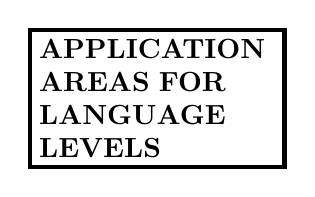
\begin{tikzpicture}[every node/.style={draw,ultra thick,text width=3cm,minimum width=3cm}]
\node{\textbf{APPLICATION\\ AREAS FOR\\ LANGUAGE\\ LEVELS}};
\end{tikzpicture}
\end{wrapfigure}
Applications better suited to high-level languages are those which require large memories. If, as in a valve controller, electronic game, appliance controller, or small instrument. the cost of a single memory chip is important. then the inefficiency of high-level languages is intolerable. If, on the other hand, as in a terminal or test equipment. the system has many thousands of bytes of memory anyway, the inefficiency of high-level languages is not as important. Clearly the size of the program and the volume of the product are important factors as well. A large program will greatly increase the advantages of high-level languages. On the other hand, a high-volume application will mean that fixed software development costs are not as important as memory costs that are part of each system.

\subsection*{WHICH LEVEL SHOULD YOU USE?}

\textbf{That depends on your particular application. Let us briefly note some of the factors
which may favor particular levels:}

\begin{wrapfigure}{r}{3.5cm+.6666em+.8pt}

\begin{tikzpicture}[every node/.style={draw,ultra thick,text width=3.5cm,minimum width=3.5cm}]
\node{\textbf{APPLICATIONS\\ FOR MACHINE\\ LANGUAGE}};
\end{tikzpicture}
\end{wrapfigure}
\textbf{Machine Language:}
\begin{wrapfigure}{r}{3.5cm+.6666em+.8pt}

\begin{tikzpicture}[every node/.style={draw,ultra thick,text width=3.5cm,minimum width=3.5cm}]
\node{\textbf{APPLICATIONS\\ FOR ASSEMBLY\\ LANGUAGES}};
\end{tikzpicture}
\end{wrapfigure}
\begin{itemize}
\item\textbf{Virtually no one programs in machine language because it is inefficient and difficult to document. An assembler costs very little and greatly reduces programming time.}
\end{itemize}

\textbf{Assembly Language:}
\begin{itemize}
\item\textbf{Short to moderate-sized programs}
\item\textbf{Applications where memory cost is a factor}
\item\textbf{Real-time control applications}
\item\textbf{Limited data processing}
\item\textbf{High-volume applications}
\item\textbf{Applications involving more input/output or control than computation}
\end{itemize}

\begin{wrapfigure}{r}{3.8cm+.6666em+.8pt}

\begin{tikzpicture}[every node/.style={draw,ultra thick,text width=3.8cm,minimum width=3.8cm}]
\node{\textbf{APPLICATIONS\\ FOR HIGH-LEVEL\\ LANGUAGES}};
\end{tikzpicture}
\end{wrapfigure}
\textbf{High Level Languages:}
\begin{itemize}
\item\textbf{Long programs}
\item\textbf{Low-volume applications requiring long programs}
\item\textbf{Applications where the amount of memory required is already very large}
\item\textbf{Applications involving more computation than input/output or control}
\item\textbf{Compatibility with similar applications using larger computers}
\item\textbf{Availability of specific programs in a high-level language which can be used in the application}
\end{itemize}

Many other factors are also important. such as the availability of a larger computer for use in development. experience with particular languages. and compatibility with other applications.

If hardware will ultimately be the largest cost in your application. or if speed is critical. you should favor assembly language. But be prepared to spend extra time in software development in exchange for lower memory costs and higher execution speeds. If software will be the largest cost in your application. you should favor a high-level language. But be prepared to spend the extra money required for the supporting hardware and software.

Of course. no one except some theorists will object if you use both assembly and highlevel languages. You can write the program originally in a high-level language and then patch some sections in assembly language. 7 However. most users prefer not to do this because of the havoc it creates in debugging. testing. and documentation

\subsection*{HOW ABOUT THE FUTURE?}

\begin{wrapfigure}{r}{3.8cm+.6666em+.8pt}

\begin{tikzpicture}[every node/.style={draw,ultra thick,text width=3.8cm,minimum width=3.8cm}]
\node{\textbf{FUTURE TRENDS\\ IN LANGUAGE\\ LEVELS}};
\end{tikzpicture}
\end{wrapfigure}
\textbf{We expect that the future will favor high-Ievellaiiguages for the following reasons:}
\begin{itemize}
\item{Programs always seem to add extra features and grow larger}
\item{Hardware and memory are becoming less expensive}
\item{Software and programmers are becoming more expensive}
\item{Memory chips are becoming available in larger sizes. at lower "per bit" cost. so actual savings in chips are less likely}
\item{More suitable and more efficient high-level languages are being developed}
\item{More standardization of high-level languages will occur}
\end{itemize}

Assembly language programming of microprocessors will not be a dying art any more than it is now for large computers. But longer programs. cheaper memory. and more expensive programmers will make software costs a larger part of most applications. The edge in many applications will therefore go to high-level languages.

\subsection*{WHY THIS BOOK?}
\textbf{If the future would seem to favor high-level languages, why have a book on assembly language programming? The reasons are:}
\begin{enumerate}
\item{Most current microcomputer users program in assembly language (almost two thirds. according to one recent survey).}
\item{Many microcomputer users will continue to program in assembly language since they need the detailed control that it provides.}
\item{No suitable high-level language has yet become widely available or standardized.}
\item{Many applications require the efficiency of assembly language.}
\item{An understanding of assembly language can help in evaluating high-level
languages.}
\end{enumerate}

The rest of this book will deal exclusively with assemblers and assembly language programming. However. we do want readers to know that assembly language is not the only alternative. You should watch for new developments that may significantly reduce
\pagebreak
\section*{REFERENCES}
\begin{enumerate}
\item{A. Osborne, \underline{An Introduction to Microcomputers: Volume 1 - Basic Concepts}, Osborne/McGraw-HilI. Berkeley, CA., 1976.}
\item{M. H. Halstead, \underline{Elements of Software Science}, American Elsevier, New York, 1977.}
\item{V. Schneider, "Prediction of Software Effort and Project Duration," \underline{SIGPLAN Notices}, June 1978, pp. 49-55.}
\item{M. Phister Jr.. \underline{Data Processing Technology and Economics}, Santa Monica Publishing Co., Santa Monica, CA. 1976.}
\item{Albrecht. Finkel. and Brown, \underline{BASIC for Home Computers}, Wiley, New York, 1978.}
\item{K. L. Bowles, \underline{Microcomputer Problem Solving Using PASCAL}. Springer-Verlag. New York, 1977.}
\item{D. D. McCracken, \underline{A Guide to PL'M Programming for Microcomputer Applications}. Addison-Wesley, Reading, Mass.. 1978.}
\item{P. Caudill. "Using Assembly Coding to Optimize High-Level Language Programs," \underline{Electronics}, February 1. 1979, pp. 121-124.}
\end{enumerate}

\end{document}